\chapter{LOS Channel - Wideband Analysis}
\label{chap:los_wide}

The analysis now transitions to the wideband case, where the signal's bandwidth is significant and can no longer be neglected. This requires moving from the narrowband model to models that explicitly account for the channel's behavior across the frequency band and in the time-delay domain.

\section{Impulse Response and Transfer Function}
For a single LOS ray, the physical channel is characterized by a single propagation path with delay $\tau_1$ and complex amplitude $\alpha_1$. The impulse response and transfer function are the same as those derived in the narrowband analysis, as they represent the underlying physical reality of the channel independent of signal bandwidth.

The physical impulse response is a single Dirac delta function, representing the instantaneous arrival of the signal after a delay $\tau_1$:
\begin{equation}
	h(\tau) = \alpha_1 \delta(\tau - \tau_1) = \left( j \frac{\lambda Z_0}{4\pi^2 R_a d_1} e^{-j2\pi f_c \tau_1} \right) \delta(\tau - \tau_1)
	\label{eq:los_impulse_response_wide}
\end{equation}
The corresponding transfer function, obtained via the Fourier transform of $h(\tau)$, is:
\begin{equation}
	H(f) = \alpha_1 e^{-j2\pi f \tau_1} = j \frac{\lambda Z_0}{4\pi^2 R_a d_1} e^{-j2\pi (f_c + f) \tau_1}
	\label{eq:los_transfer_function_wide}
\end{equation}
The magnitude of the impulse response is a single impulse, as shown in Figure \ref{fig:h_tau_los}. The magnitude of the transfer function, $|H(f)| = |\alpha_1|$, is constant across all frequencies, confirming that the LOS channel is frequency-flat, as depicted in Figure \ref{fig:Hf_los}.

\begin{figure}
	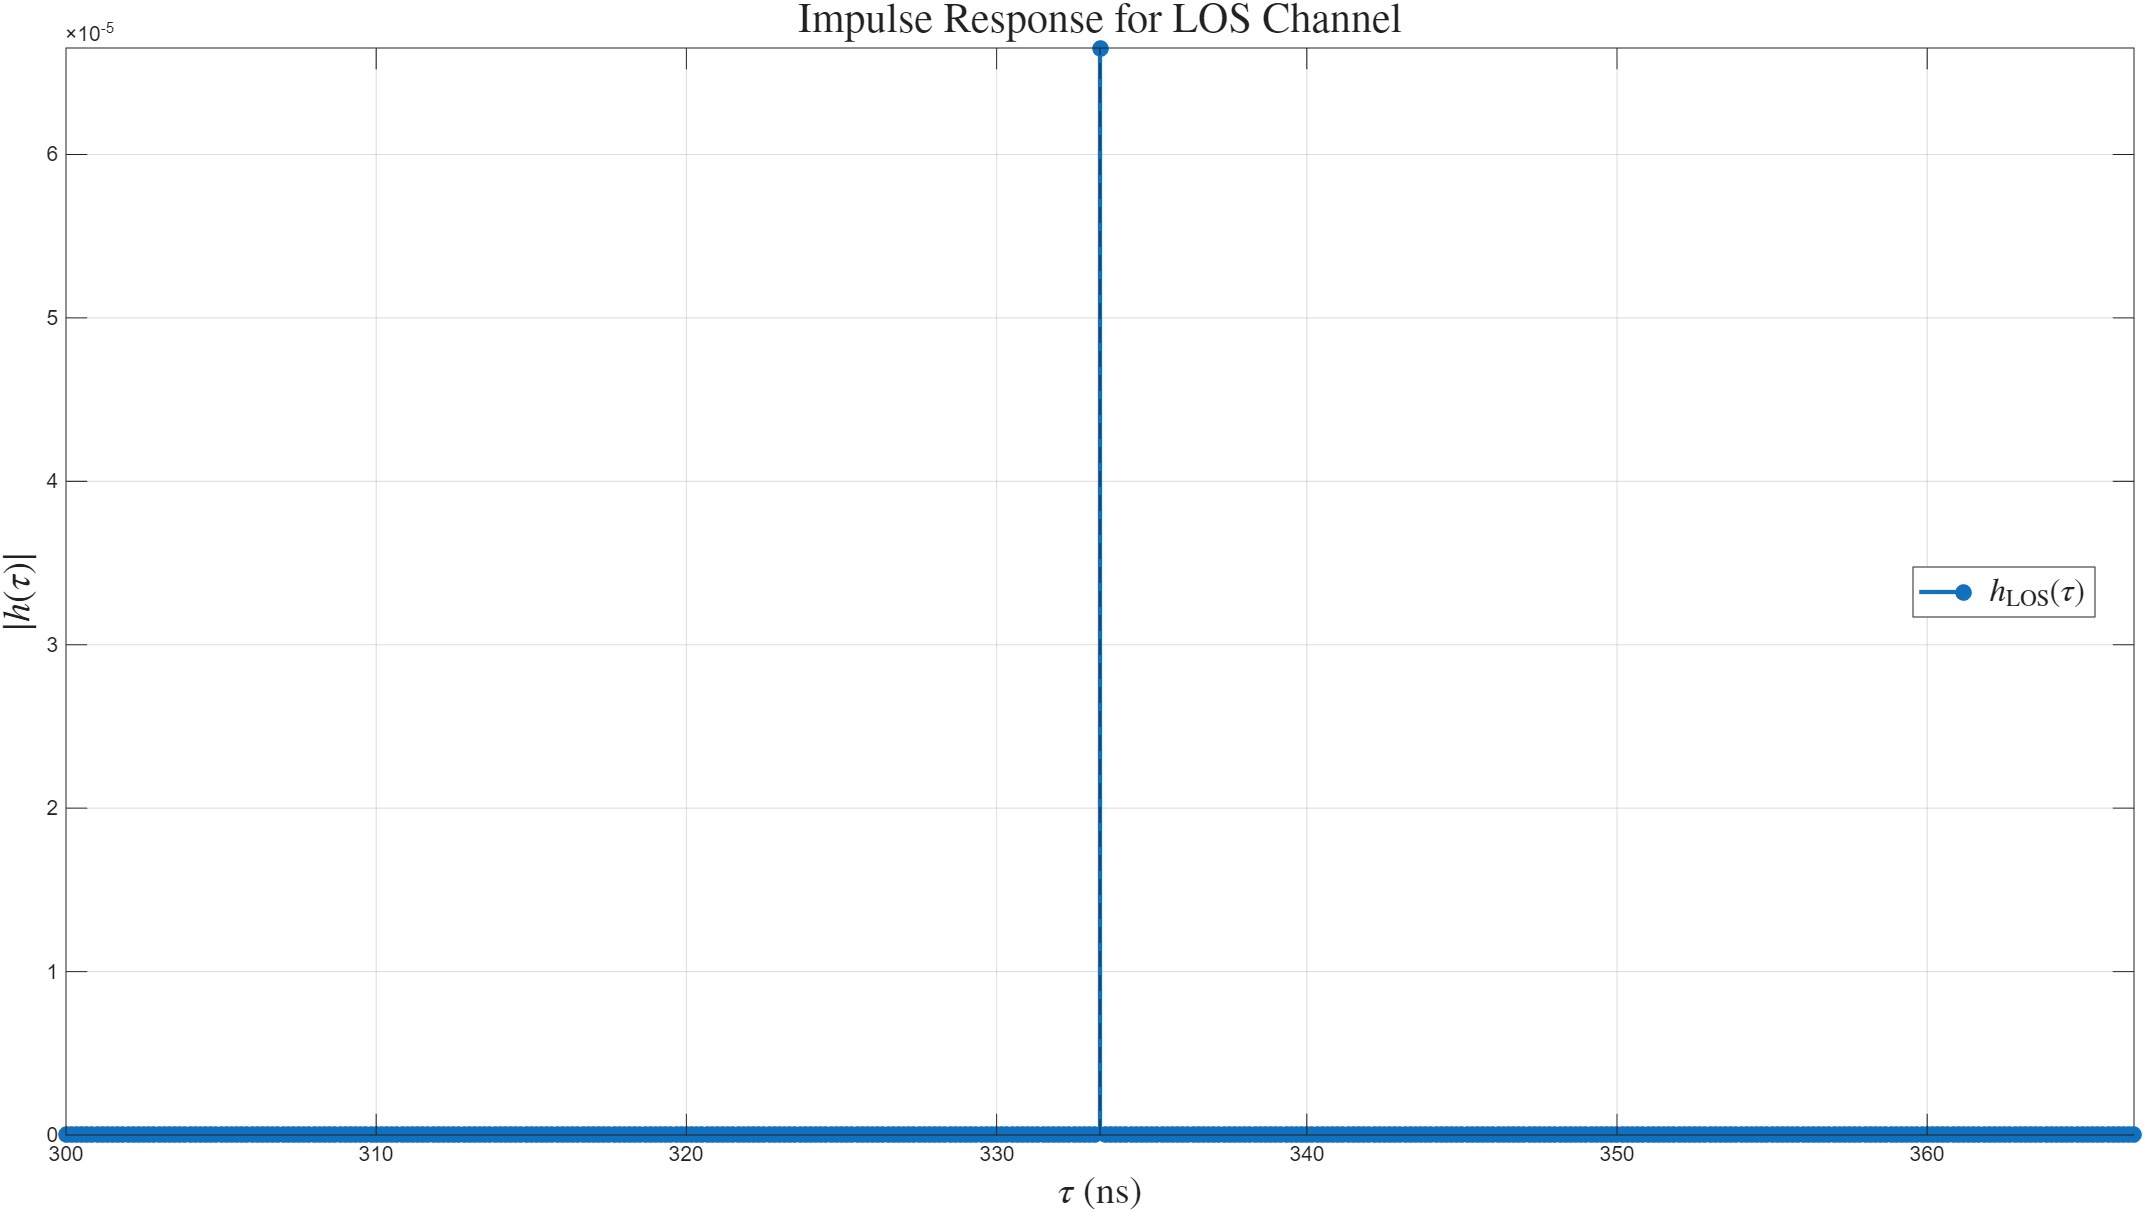
\includegraphics[width=\linewidth]{"content/4-images/h-tau-LOS.png"}
	\caption{Physical impulse response $|h(\tau)|$ for the LOS channel at $d=100$ m. The single impulse occurs at $\tau_1 = 333.33$ ns.}
	\label{fig:h_tau_los}
\end{figure}

\begin{figure}
	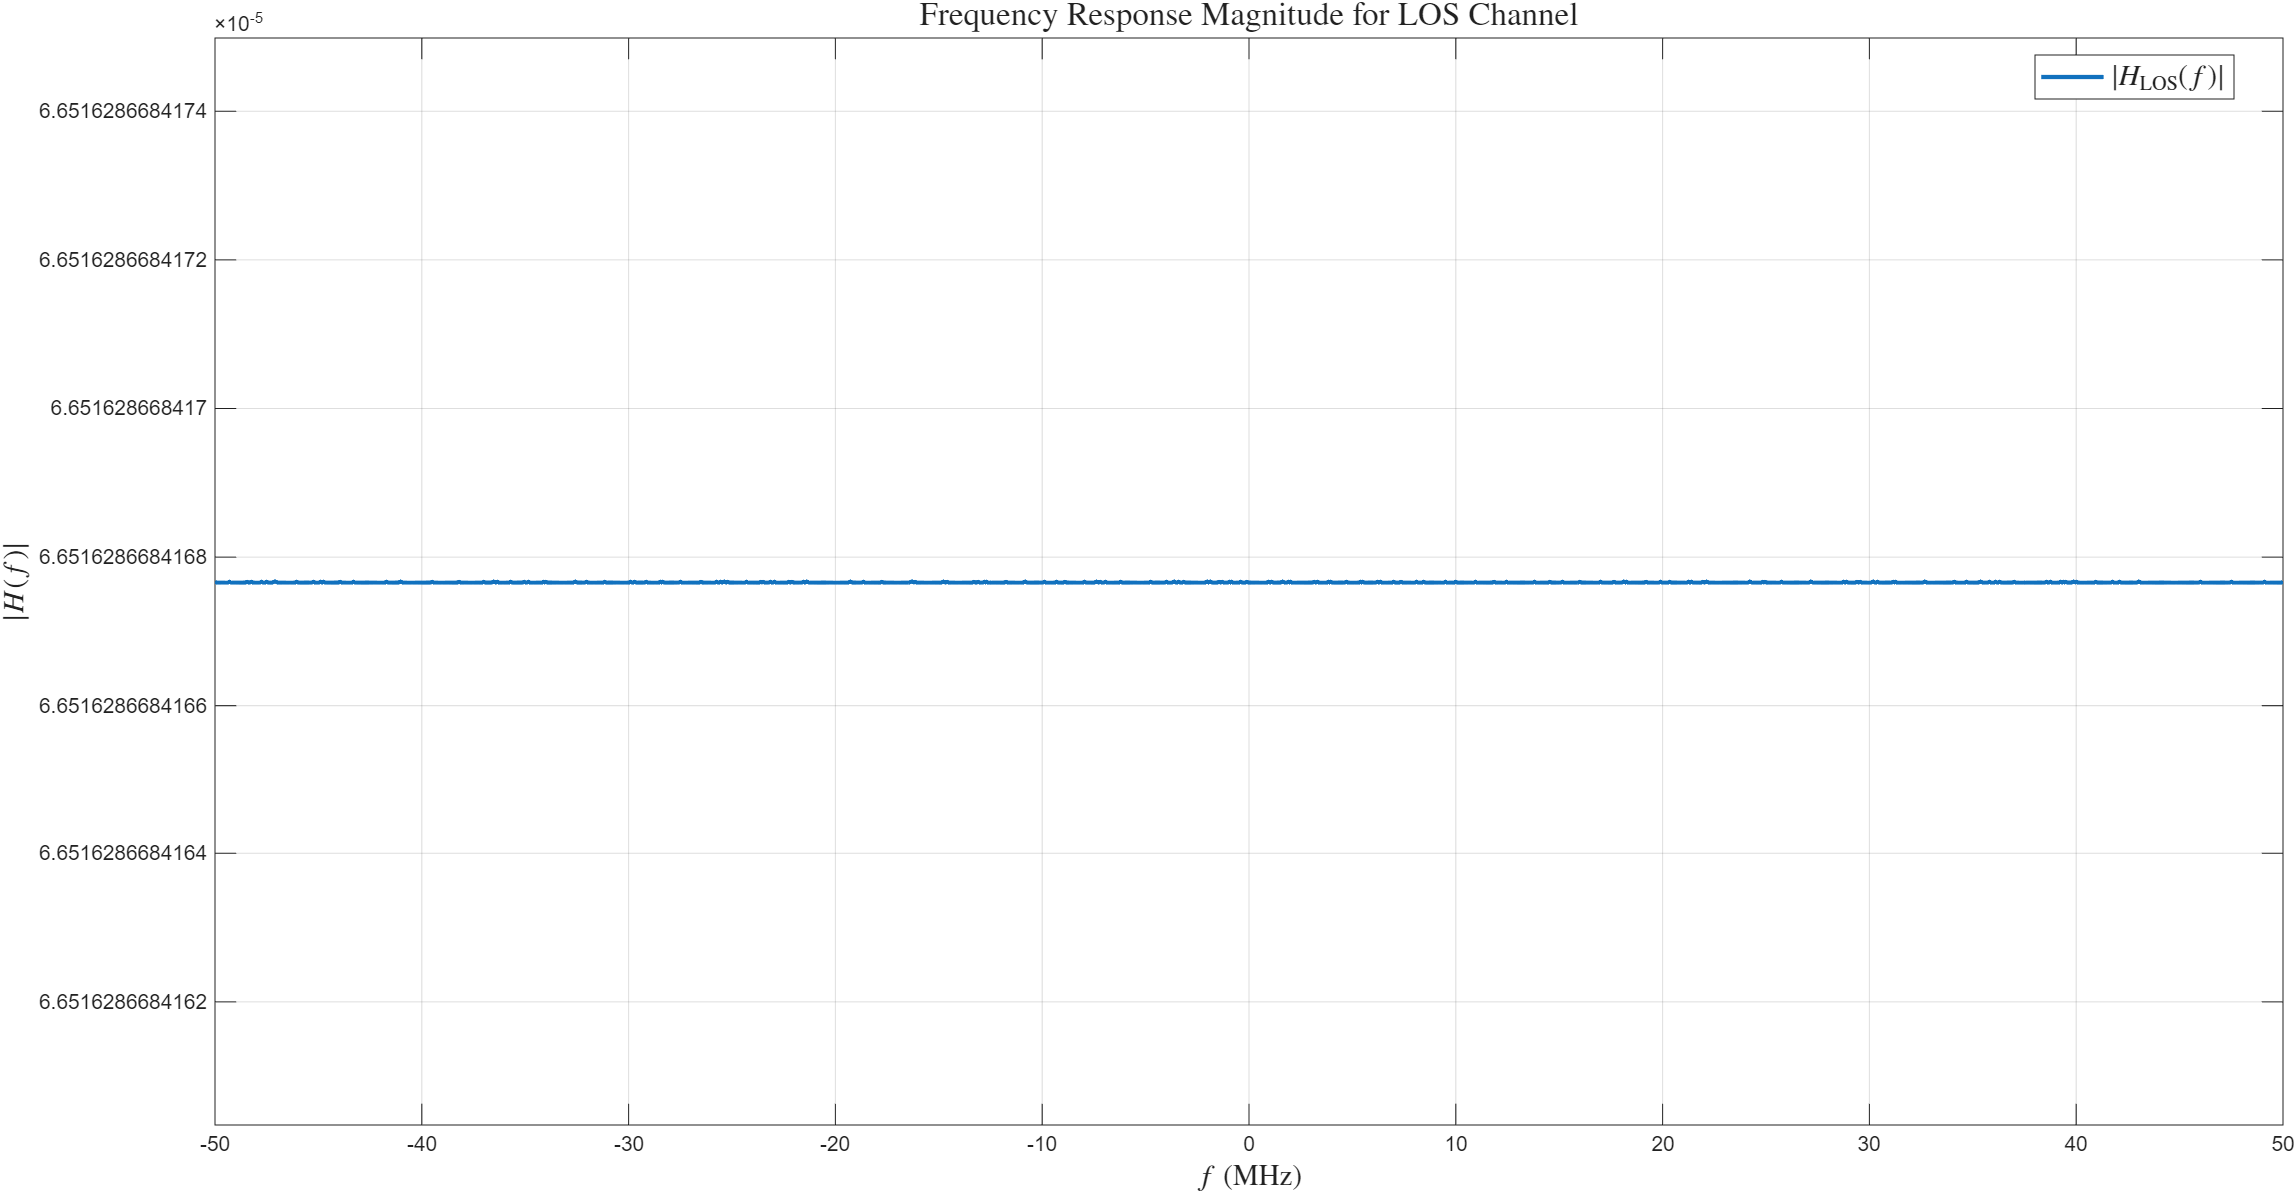
\includegraphics[width=\linewidth]{"content/4-images/Frequency Response H(f) - LOS.png"}
	\caption{Transfer function magnitude $|H(f)|$ for the LOS channel. The response is flat across the entire bandwidth.}
	\label{fig:Hf_los}
\end{figure}


\section{Tapped Delay Line Model $h_{TDL}(\tau)$}
The Tapped Delay Line model provides a discrete-time representation of the channel that accounts for the finite bandwidth $B$ of the communication system. The time resolution of the system is $\Delta\tau = 1/B$. The TDL impulse response is given by:
\begin{equation}
	h_{TDL}(\tau) = \sum_{l=0}^{L} h_l \delta(\tau - l\Delta\tau)
\end{equation}
where the complex gain of the $l$-th tap, $h_l$, is calculated by projecting the physical impulse response onto a basis of sinc functions:
\begin{equation}
	h_l = \int_0^{\infty} h(\tau) \operatorname{sinc}(B(\tau-l \Delta \tau)) d \tau
\end{equation}
Substituting the physical impulse response for the LOS channel, $h(\tau) = \alpha_1 \delta(\tau - \tau_1)$, into this integral gives:
\begin{equation}
	h_l = \int_0^{\infty} \alpha_1 \delta(\tau - \tau_1) \operatorname{sinc}(B(\tau-l \Delta \tau)) d \tau
\end{equation}
Using the sifting property of the Dirac delta function, the expression for the tap gains simplifies to:
\begin{equation}
	h_l = \alpha_1 \operatorname{sinc}(B(\tau_1 - l \Delta \tau))
\end{equation}
This equation shows that the gain of each tap is determined by the value of a sinc function centered at the physical delay $\tau_1$. For the simulation parameters ($B=100$ MHz, $\Delta\tau = 10$ ns), the LOS delay $\tau_1 = 333.33$ ns falls between the 33rd and 34th taps. The sinc function's main lobe will distribute the energy of the physical ray primarily across these adjacent taps, with smaller contributions to other taps, as shown in Figure \ref{fig:h_tdl_los}.

\begin{figure}[h!]
	\centering
	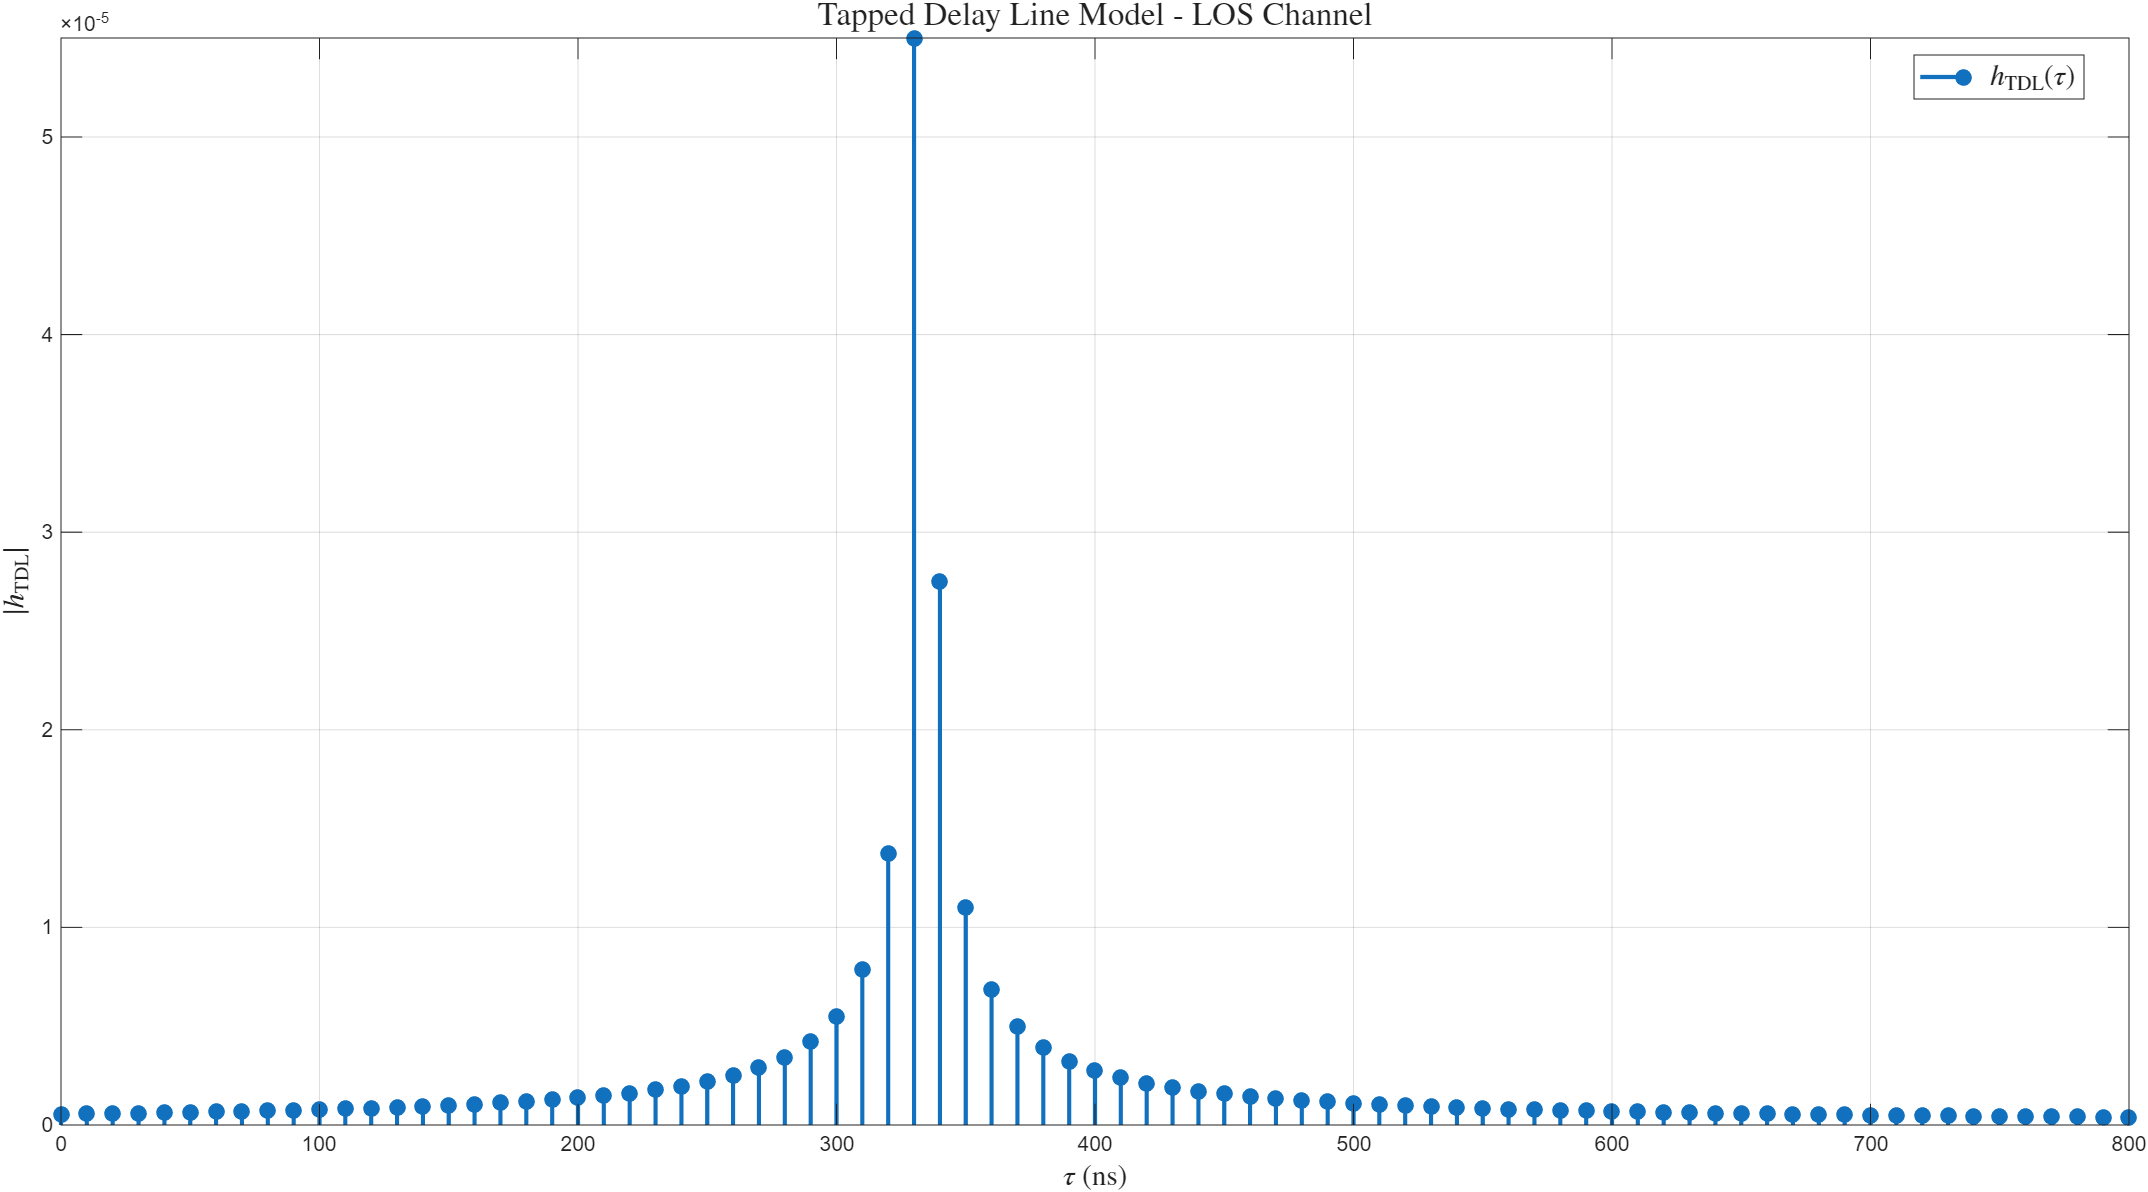
\includegraphics[width=\linewidth]{"content/4-images/Tapped Delay Line Model - LOS Channel.png"}
	\caption{Tapped Delay Line model $|h_{TDL}(\tau)|$ for the LOS channel. The energy of the single physical ray is spread across several discrete taps centered around the true delay $\tau_1$.}
	\label{fig:h_tdl_los}
\end{figure}

\section{Interpretation of Results}
The wideband analysis of the LOS channel provides several key insights:
\begin{itemize}
	\item \textbf{No Time Dispersion:} The physical impulse response consists of a single, sharp impulse. This signifies that there is no time dispersion in the channel; a transmitted impulse arrives as a single impulse at the receiver, albeit delayed and attenuated. This is the ideal channel condition.
	\item \textbf{Frequency-Flat Fading:} The lack of time dispersion directly results in a frequency-flat transfer function. Since $|H(f)|$ is constant, all frequency components of the transmitted signal are attenuated equally. The channel does not introduce any spectral distortion, which simplifies receiver design significantly.
	\item \textbf{TDL as a Band-Limited Model:} The TDL model illustrates the effect of the system's finite bandwidth. While the physical ray arrives at a precise moment $\tau_1$, the system with its limited time resolution $\Delta\tau$ perceives this energy as being spread across several discrete time intervals (taps). The sinc interpolation correctly models this effect, showing that the power is not confined to a single tap unless the physical delay happens to be an exact multiple of $\Delta\tau$.
\end{itemize}
